\section{Deviations from the ideal gas equation}
    
    Real gases exhibit behaviour that departs from the predictions of the ideal gas equation, especially under conditions of high pressure and low temperature. These deviations arise mainly due to intermolecular forces and the finite size of gas molecules: two factors neglected in the ideal gas model. Understanding these departures is important because most practical gases behave non-ideally under ordinary laboratory conditions.
    
    Real gases fail to obey the ideal gas law, $PV=nRT$, when intermolecular interactions and finite molecular volumes become significant. At high pressures and low temperatures, gases show noticeable departures from ideality, often represented using $PV$ vs $P$ or \textit{compressibility factor} $Z=\dfrac{PV}{RT}$. These deviations provide important clues about the underlying physics governing real gas behaviour.
    
    \subsection{The virial equation}
    	The virial equation provides a systematic, low-density expansion of a real gas's equation of state and quantifies departures from ideal behaviour in terms of temperature-dependent coefficients. Each virial coefficient encodes the contribution of clusters of a given size -- two-body, three-body, etc. -- so the series links macroscopic thermodynamics to microscopic intermolecular forces. It is most useful for dilute gases where truncation after the first few terms gives accurate results; it breaks down when density is high or near phase transitions.
    
	    We write the compressibility factor as
	    \begin{align*}
	    	Z=\dfrac{PV_m}{RT}
	    \end{align*}
	    where $V_m$ is the molar volume.
	    
	    Then the virial expansion in powers of the molar density $\rho\equiv\dfrac{1}{V_m}$ is
	    \begin{align*}
	    	\boxed{Z=1+B(T)\rho+C(T)\rho^2+D(T)\rho^3+\cdots}
	    \end{align*}
	    or equivalently, as an expansion in inverse molar volume:
	    \begin{align*}
	    	\boxed{Z=1+\dfrac{B(T)}{V_m}+\dfrac{C(T)}{V_m^2}+\dfrac{D(T)}{V_m^3}+\cdots}
	    \end{align*}
	    Here $B(T)$, $C(T)$, $\dots$ are the molar virial coefficients: $B$ is the second virial coefficient (pair interactions), $C$ the third (three-body effects), and so on.
	    
	\subsection{Andrew's experiments on \ce{CO2} gas}
		Andrew's experiments provided the first systematic evidence of the non-ideal behaviour of real gases. By studying the isotherms of \ce{CO2}, he demonstrated that gases do not liquefy merely by applying pressure unless their temperature is below a certain critical value. His work revealed the presence of characteristic flat portions of isotherms -- signifying phase coexistence -- which the ideal gas equation cannot predict. These experiments paved the way for the development of modern real-gas equations of state.
	
		\subsubsection{Description of Andrew's isotherms}
			For \ce{CO2}, Andrew plotted $P$-$V$ isotherms at different temperatures.
			\begin{figure}[h!]
				\centering
				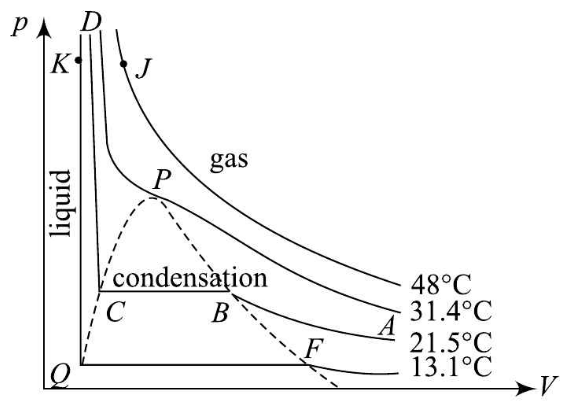
\includegraphics[width=0.45\textwidth]{figures/fig_andrews-plot.png}
			\end{figure}
			\begin{itemize}
				\item Above a certain temperature, the isotherms resemble smooth curves similar to ideal behaviour.
				\item Below that temperature, the isotherms flatten, indicating coexistence of liquid and gas.
			\end{itemize}
			The characteristic plateau corresponds to the liquid-vapour equilibrium region. Andrew also discovered the critical isotherm, at temperature $T_c$, where the flat portion disappears, and the gas cannot be liquefied by pressure alone.
			
	\subsection{Critical constants}
		\textit{Critical constants} describe conditions under which the gas exhibits the \textit{critical point} -- a unique state where distinct liquid and gas phases cease to exist. At this point, the properties of the liquid and vapour become identical. These constants are essential for understanding gas–liquid transitions and for deriving real-gas equations. They are determined experimentally from $P$-$V$ isotherms.
		
		The three critical constants are:
		\begin{enumerate}
			\item \emph{Critical temperature} $T_c$ -- the maximum temperature at which a gas can be liquefied by pressure alone.
			
			\item \emph{Critical pressure} $P_c$ -- the pressure required to liquefy a gas at $T_c$
			
			\item \emph{Critical volume} $V_c$ -- the molar volume at the critical point
		\end{enumerate}
		
		At the critical point, the isotherm satisfies the following conditions:
		\begin{align*}
			\qty(\pdv{P}{V})_{T_c}=0\qq{and}\qty(\pdv[2]{P}{V})_{T_c}=0
		\end{align*}
		
	\subsection{Continuity of liquid and gaseous state}
		The concept of continuity emphasises that liquid and gaseous states are not fundamentally distinct but represent different regions of the same phase. As Andrew’s isotherms show, one can move from a gas-like state to a liquid-like state without crossing a phase boundary -- provided the temperature remains above the critical temperature. This insight marks a major departure from earlier ideas that regarded gases and liquids as entirely different. It also supports the modern view that phases are defined by thermodynamic properties, not by intrinsic physical differences.
		
		Above $T_c$, continuous compression transforms a gaseous state smoothly into a highly compressed fluid without condensation. This region is often called the supercritical fluid region, where properties interpolate between liquid-like and gas-like characteristics.
		
	\subsection{Boyle temperature}
		The Boyle temperature represents the temperature at which a real gas shows minimal deviation from ideal behaviour over a moderate range of pressures. It serves as a useful reference for identifying temperatures at which intermolecular attractions and repulsions cancel out. At this temperature, the compressibility factor $Z\approx 1$ for a substantial pressure range. Thus the Boyle temperature is significant for gas approximation models.
		
		The Boyle temperature $T_B$ is defined using the compressibility factor expansion of the virial equation:
		\begin{align*}
			Z=1+B(T)\dfrac{1}{V_m}+C(T)\dfrac{1}{V_m^2}+\cdots
		\end{align*}
		At Boyle temperature $T_B$, $B(T_B)=0$ and so the second virial term vanishes. This means that, at the Boyle temperature, the pair-wise interactions do not occur anymore.